%%%%(c)
%%%%(c)  This file is a portion of the source for the textbook
%%%%(c)
%%%%(c)    Abstract Algebra: Theory and Applications
%%%%(c)    Copyright 1997 by Thomas W. Judson
%%%%(c)
%%%%(c)  See the file COPYING.txt for copying conditions
%%%%(c)
%%%%(c)
\chap{Further topics in Cryptography}{Crypto}
\section{Diffie Hellman Key Exchange}\label{sec:DHKE:1}

In order to share a private message over a public domain a sender must  "lock" or encrypt their message using a \emph{key}\index{key! in cryptogaphy}.  Recall from Section \ref{sec:crypt:overview}, that in cryptography a  key is a special piece of information (usually a number)  that is required to encrypt and decrypt data which is shared between the sender and receiver. There are generally three types of keys used: public, private and symmetric keys. A \emph{Public Key}\index{Public Key! in cryptography} can be widely distributed, and is used for encrypting messages.  A\emph{Private Key}\index{Private Key! in cryptography} is only known to the sender, and is used for decrypting messages (it can also be used for encrypting messages when using cryptosystems such as RSA).  Finally, a \emph{Symmetric Key}\index{Symmetric Key! in cryptography} is known by the sender and receiver, and is used to encypt and decrypt messages.  Not all cryptosystems require all three kinds of keys, but every cryptosystem must have either a private key or a symmetric key.

  If a symmetric key is used, then both parties must share their key before they can begin communicating securely. The requirement of establishing a key exchange is so essential that it is embedded into almost every technology we use today.  Some examples of key exchange can be seen in media applications, cell phones, banking, online purchasing, and emails.  

 But what if the only way the two parties have to communicate is via a public network (such as the Internet), where eavesdroppers can listen in?  Under these conditions how can they possibly establish a shared key in such a way that no one else can find out?  The Diffie Hellman Key Exchange (DHKE) is one possible solution to the problem of creating a secret key over an insecure communication channel.  Note that the DHKE is not used for encryption/decryption of messages, but only to establish a key that can be used to encrypt/decrypt subsequent messages.  Follow the steps below to see the DHKE process.  

 \begin{enumerate}[Step 1.]
 \item First, Moses and Rachael agree upon a pair of numbers $p$ and $g$. $p$ is called the \term{modulus},while $g$ is called the \term{base}. These numbers are not secret, and Moses and Rachael don't care if eavesdroppers find out what $p$ and $g$ are. In practice $p$ and $g$ are required to have certain properties (as explained below) to maximize secrecy.  However, the DHKE procedure still works for any values of $p$ and $g$.
\item Moses chooses a secret integer $n$, known only to himself.  He then computes $q$ where $q =\bmod(g^n,p)$, and sends Rachael the value of $q$. Rachael does not need to know the value of $n$.
\item Rachael similiarly chooses her own secret integer $m$, computes $r$ where $r =\bmod(g^m,p)$ and sends Moses the value of $r$.
\item Moses computes $ \bmod (r^n , p ) = K_1$;
\item Rachael computes $ \bmod (q^m , p ) = K_2$;
\end{enumerate} 
It turns out that when $K_1$ and $K_2$ are computed by the above procedure, then $K_1$ is always equal to $K_2$.  You will show this in the next exercise.  
\begin{figure}[htb]
	   \center{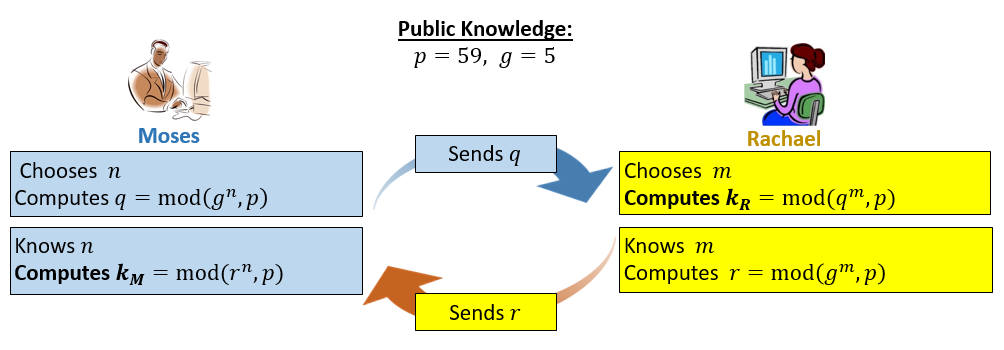
\includegraphics[width=5.5in]
	         {images/DHKE_1.png}}
	  \caption{\label{fig:DH:DHKE_1} Key exchange between Moses and Rachael using DHKE}
\end{figure}

\begin{exercise}{k1isk2}\\
Fill in the blanks in the following proof that  $K_1$ is always equal to  $K_2$.\\
  	\begin{proof} 
		\begin{align*} 
		K_1 &=   \bmod (r^n , \underline{~~~~~~}) 
           	\\&=  \bmod ( \underline{~~~~}^{\underline{~~~~~~}} , p) , p )&& \text{(substitution)}	%ans: \bmod ( \bmod (g^m , p)^n , p )&& \text{(substitution)}
		\\&= \bmod ( \bmod ((g^{\underline{~~~~~~}}) , p) , p )&&  \text{(rules of exponents)}	%ans: \bmod ( \bmod ((g^{mn}) , p) , p )&&  \text{(rules of exponents)}	
           	\\&= \bmod ( \bmod ((\underline{~~~~~~})^{\underline{~~~~~~}} , p) , p )  &&\text{(rules of exponents)}	%ans:  \bmod ( \bmod ((g^n)^m , p) , p )  &&\text{(rules of exponents)}
           	\\&= \bmod (\underline{~~~~~~}^m , p )&&\text{(substitution)}   	%ans: \bmod ( \bmod ((g^n , p)^m , p )&&\text{(substitution)}
		\\&= K_2
		\end{align*} 
   	Thus, $K_1 = K_2 = K$ is a symmetric key.\\

  	\end{proof}
\end{exercise}

Now that you understand the process for DHKE, follow the example below.  (Note that this example is just to give you the idea--it's much too simple to use in practical applications.)

 \begin{eg} Key Exchange between a sender and receiver (Moses and Rachael) using the DHKE is shown in the following steps.
\begin{enumerate}[Step 1.]
\item Prior to sending data, Moses and Rachael agree $p$ = 13 and $g$= 7; 
\item Moses chooses $n$ = 2, and sends Rachael $\bmod (7^2 , 13) = 10$;
\item Rachael chooses $m$ = 8, and sends Moses $\bmod (7^8  , 13) = 3 $;
\item Moses computes $\bmod ((3)^2 , 13 ) = 9$;
\item Rachael computes $\bmod ((10)^8 , 13 ) = 9$;
\item Moses and Rachael share the number 9;
\end{enumerate}
\end{eg}

%  \emph{Fermat's Little Theorem}\index{Fermat's Little Theorem! in cryptography} states that if $p$ is a prime number such that $p \nmid a$, and $a$ is an integer, then $1 \equiv \bmod(a^{p-1}, p)$.

%\begin{eg} Let $p = 5$ and $a = 1, 2, 3, 4 \text{ and } 5$
%$$ 5 \nmid 1 \implies \bmod(1^{5-1}, 5) \equiv 1$$
%$$ \bmod(1^{4}, 5) \equiv 1$$
%$$ \bmod(1, 5) \equiv 1$$
%$$ 5 \nmid 2 \implies \bmod(2^{5-1}, 5) \equiv 1$$
%$$ \bmod(2^{4}, 5) \equiv 1$$
%$$ \bmod(16, 5) \equiv 1$$
%$$ 5 \nmid 3 \implies \bmod(3^{5-1}, 5) \equiv 1$$
%$$ \bmod(3^{4}, 5) \equiv 1$$
%$$ \bmod(18	, 5) \equiv 1$$
%$$ 5 \nmid 4 \implies \bmod(4^{5-1}, 5) \equiv 1$$
%$$ \bmod(4^{4}, 5) \equiv 1$$
%$$ \bmod(256, 5) \equiv 1$$
%$$ 5 | 5 \text { (so the theorem does not apply)}$$
%$$ \bmod(5^{5-1}, 5) \equiv 0$$

%Since all values of $a$ such that $1 \leq a \leq p$ are congruent to $1$, then Fermat's Little Theorem tells us that $p$ is prime, but are there numbers that exist that pass Fermat's Little Theorem but are not prime?  The answer is yes, these numbers are called \emph{Lucas-Carmichael Numbers}\index{Lucas-Carmichael Numbers! in cryptogaphy}.  (or \emph{pseudoprimes}\index{Pseudoprimes}) 

Following the example above you can see that the DHKE requires that you raise a given number $g$ to a natural number (either $m$ or $n$) and take the result mod $p$. This operation is called \term{discrete exponentiation}. Calculating discrete exponentials with small values of $m$ or $n$ is manageable, but in practice the exponent $m$ or $n$ can be enormous, with hundreds of digits. It would seem that in this case discrete exponentiation would take a long, long time to compute.  But we can use the repeated squaring formula described in Section \ref{exercise:crypt:power} to speed up the process.  

You may create a spreadsheet using the repeated squaring formula (or use \url{www.wolframalpha.com}) to find answers to the following exercises.
 
\begin{exer}
Given $p$ = 32452867; $g$ = 54321; and $n$ = 876.  
\begin{enumerate}[(a)]
\item What number do you send?  
%ans: mod((54321)876, 32,452,867) = 19,439,625

\item Alice sends back 31975948.  What is your shared key with Alice? 
%ans: K = mod((31,975,948)876, 32,452,867) = 16,045,878

\item  Bob receives your number from (a) and chooses $m$ = 127. What number does he send back to you? And what is your shared key with Bob?
%ans: K = mod((19,439,625)124, 32,452,867) = 22721372

\item
By an amazingly lucky chance, Alice's choice of $m$ just happens to be very close to Bob's choice.  What is Alice's choice of $m$?
\end{enumerate}
\end{exer}

\begin{exer}
Given $p$ = 86028157; $g$ = 98765; and $n$ = 123.  
\begin{enumerate}[(a)]
\item	What number do you send?  
%ans: mod((98765)123, 86,028,157) = 7,262,961

\item Carol sends back 53161396. What is your shared key? 
%ans: K = mod((53,161,396)123, 86,028,157) = 35,164,864

\item Deborah receives your number from (a) and chooses $m$ = 81. what number does she send to you? And what is your shared key with Deborah?
% K = 5998268

\item
By an extraordinarily lucky chance, Deborah's choice of $m$ just happens to be not too far from Carol's choice.  What is Carol's choice of $m$?
% 87

%ans: K = mod((7,262,961)87, 86,028,157) = 35,164,864
\end{enumerate}
\end{exer}
Now that we understand the DHKE process, let's try to understand why it effectively guarantees the secrecy of the shared key. First, we need to understand a little more about the operation of discrete exponentiation, which (as we've seen) is the foundation of the DHKE process. So we're going on a short digression, but don't worry--we'll get back to the main point shortly. 

In previous math courses you learned that the inverse operation of exponentiation is taking the logarithm: for example, $2^3 = 8$ while $\log_{2}8 = 3$.  It's possible to do the same with discrete exponentiation: the inverse operation to discrete exponentiation is  called \term{discrete logarithm} or (DL). Note that since discrete exponentiation involves raising to a power which is a natural number, the DL will always be a natural number.   For example, since $\bmod(2^5,7)=4$, we could say that under multiplication mod 7,  $5$ is a DL  of $4$ with base $2$. Now why did we say, ``\emph{a} DL'' rather than ``\emph{the} DL''? Because  there happens to be more than one:

\begin{exercise}{DLex1}
\begin{enumerate}[(a)]
\item
Find all natural numbers $n$ such that $\bmod(2^n,7)=4$.  Use your result to complete the following sentence: ``Under multiplication mod 7, the discrete logarithm(s) of $4$ with base 2  are \ldots.''
\item
Find all natural numbers $n$ such that $\bmod(2^n,7)=3$.  Use your result to complete the following sentence:  ``Under multiplication mod 7, the discrete logarithm(s) of $3$ with base 2 are \ldots.''
\item
Find all nonzero elements of $\mathbb{Z}_7 \setminus \{0\}$ which have no discrete logarithms with base 2.
\item
Find all nonzero elements of $\mathbb{Z}_7 \setminus \{0\}$ which have no discrete logarithms with base 3.
\end{enumerate}
\end{exercise}

The preceding exercise points out some key issues with discrete logarithms. Sometimes there are lots of them, and sometimes there aren't any! These phenomena are related to the one-to-oneness and ontoness properties of  the discrete exponential function (recall Definitions~\ref{121defn} and \ref{ontoDef}, respectively):

\begin{exercise}{DLex2}
\begin{enumerate}[(a)]
\item
We may define a function $f: \mathbb{N} \rightarrow \mathbb{Z}_7 \setminus \{0\}$ by the equation: $f(n) = \bmod(2^n,7)$. 
Use parts (a) and (b) of Exercise~\ref{exercise:Crypto:DLex1} to prove that $f$ is neither one-to-one nor onto.
\item
We may also define a function $g: \mathbb{N} \rightarrow \mathbb{Z}_7 \setminus \{0\}$ by the equation: $f(n) = \bmod(3^n,7)$. 
Prove or disprove: $g$ is one-to-one.
\item
With the same $g$ as in part (b), prove or disprove: $g$ is onto.
\end{enumerate}
\end{exercise}

This exercise suggests the following question:  Under what conditions can we guarantee that the discrete exponentiation function is onto and/or one-to-one? (This turns out to be more than an idle question, as we shall see shortly.)  To gain some leverage against this problem, we'll make use of   Proposition~\ref{proposition:poly:Up_cyclic} from Chapter~\ref{poly}, which tells us that the multiplicative group $\mathbb{Z}_p\setminus \{0\}$ is \emph{cyclic}, whenever $p$ is a prime. (In Chapter~\ref{poly} we also used the notation $U(p)$ instead of $\mathbb{Z}_p\setminus \{0\}$, and we'll use this same notation in the following.) This means that for any prime $p$, there is a $g \in U(p)$  such that $g$ is a \emph{generator}\footnote{A generator of $U(p)$ is also referred to as a \term{primitive element} of $\mathbb{Z}_p$.} of  $U(p)$: that is, $U(p) = \langle g \rangle$ (recall from Chapter~\ref{groups} that for a finite group, $\langle g \rangle = \{g, g^2, g^3, \ldots \}$). 
Thus any element of $U(p)$ may be expressed as a power of $g$ (under mod $p$ multiplication).  In other words, the discrete exponentiation function $f: \mathbb{N} \rightarrow U(p)$ given by $f(n) = \bmod(g^n,p)$ is an onto function!  

It turns out that onto-ness also gives use one-to-oneness, when we restrict $f$ to the appropriate domain:

\begin{exercise}{} 
\begin{enumerate}[(a)]
\item
Define $h: U(13) \rightarrow U(13)$ by: $h(n) = \bmod(2^n,13)$.  (Note that the domain of $h$ is restricted to $U(13)$.)  Show that $h$ is a bijection.
\item
Find another number $k \in U(13)$ such that $h: U(13) \rightarrow U(13)$ given by $h(n) = \bmod(k^n,13)$ is also a bijection.
\item
Suppose that $p$ is a prime, and $g$ is a generator of $p$.  Consider the function $f: U(p) \rightarrow U(p)$ given by $f(n) = \bmod(g^n,p)$.  (Note that $f$ is the same as the discrete exponentiation function defined above, except the domain has been restricted.)  Show that $f$ is a bijection.
\end{enumerate}
\end{exercise}

It's about time we got back to the main point. Why do we even care about DL anyway? Well, suppose an eavesdropper who's listening in on Moses and Rachael's conversation wants to figure out the secret key. 
The eavesdropper knows $p, g, q=\bmod(g^n,p)$, and $r=\bmod(g^m,p)$.  This is all the information he has in order to figure out the shared key, which is  $K=\bmod(g^{mn},p)$. If he could figure out $m$ he'd be golden, because then he could compute $\bmod(q^m,p)$ which is equal to $K$. But this is none other than a DL problem, since $m$ is a DL of $r$ with base $g$ under multiplication mod $p$.  

There's an issue that we should address here. We've pointed out that any DL problem has many different solutions. What if the eavesdropper finds a different solution to the DL problem, which is not equal to the $m$ originally used by Rachael? It turns out that the eavesdropper can crack the code with \emph{any} DL solution, as the following exercise shows:

\begin{exercise}{DLex3}
We've just stated that ``$m$ is a DL of $r$ with base $g$ under multiplication mod $p$''.  But we already know there are \emph{many} DL's, not just one. Let $m'$ be a \emph{different} DL of $r$ with base $g$ under multiplication mod $p$. Show that $\bmod(g^{mn},p)=\bmod(g^{m'n},p)$. In other words, an eavesdropper can use \emph{any} DL of $r$ with base $g$ under multiplication mod $p$ to find the shared key.
\end{exercise}

\begin{exercise}{DLex4}
Suppose another eavesdropper was able to compute a DL of $q$ with base $g$ under multiplication mod $p$.  Explain how she could use this information to find Moses and Rachael's secret shared key.
\end{exercise}

The security of the DHKE leverages the easy computation of the discrete exponentials versus the difficulty of computing DL's. (A function which is easy to compute but hard to invert is referred to as a \term{one-way function}. Discrete exponentials (for suitable $p$'s and $g$'s) form a very important class of one-way functions.)
The following simple example introduces how this works in practice. 

\begin{example}{one-way}
It is easy to calculate $\bmod(2^{m},  11)$ for different values of $m$: for example, when $m =8$ then we get $\bmod(2^{8},  11) =\bmod(256,  11)  = 3$.  However, when you try to invert the process, you have: given $\bmod(2^{m},  11) = 3$, calculate $m$. There is no easy way to do this. As you can see below the results jump around, and each solution is equally likely to be an integer between 0 and 11. 
$$ \bmod(2^{1}, 11)=2$$
$$ \bmod(2^{2}, 11)=4$$
$$ \bmod(2^{3}, 11)=8$$
$$ \bmod(2^{4}, 11)=5$$
$$ \bmod(2^{5}, 11)=10$$
$$ \bmod(2^{6}, 11)=9$$
$$ \bmod(2^{7}, 11)=7$$
$$ \bmod(2^{8}, 11)=3$$
$$ \bmod(2^{9}, 11)=6$$
$$ \bmod(2^{10}, 11)=1$$
\end{example}
If you try to calculate $m$ using a brute force method (that is, computing all possible solutions one at a time), you would have to calculate 8 different solutions before you find the right answer. 

The larger the modulus, the harder the DL is to find. The exercise below is designed to show how many computations a brute force attack would take in comparison to a growing modulus.

\begin{exercise}{DLP}
Use the Repeated Square spreadsheet from Exercise \ref{exercise:crypt:power} to solve the following DL Problems. In each case, write down how many discrete exponentials you need to compute in order to find the answer.  
\begin{enumerate}[(a)]
\item Given $ \bmod(7^{m}, 41)=28$, solve for $m$.
%ans: 29

\item Given $ \bmod(5^{m}, 73)=13$, solve for $m$.
%ans: 59

\item Given $ \bmod(17^{m}, 211)=161$, solve for $m$.
%ans: 161

\item
What trend do you see in the number of computations required in parts (a), (b), (c), and how does it relate to the moduli in the different cases?
\end{enumerate}
\end{exercise}

\subsection{Man in the middle attack}
Our previous discussion indicates the DHKE is very hard to crack if it uses a large enough modulus $p$ and a suitable base $g$. But, is there any way to successfully eavesdrop on Moses and Rachael's conversation without actually cracking the code?  Both Moses and Rachael seem confident with the security the DHKE provides, since an attacker would only be privy to $\bmod (g^n , p)$ and $\bmod (g^m , p)$, each of which cannot be used to decrypt the message since an attacker would have to compute the DL problem to find $m$ and $n$. 

But, what would happen if an attacker, Fred (an eavesdropper) places himself between Moses and Rachael's messages?  If Fred could do this then Rachael's message would pass through Fred first before reaching Moses, and vice-versa. Now, Fred can intercept the public key and can establish his own private key with Moses and Rachael.  Fred is now able to read or alter messages.  This type of attack is commonly referred to as the Man in the Middle (MiM) attack.  See Figure~\ref{fig:DH:DHKE_2} to see how Fred is able to modify the Key Exchange.
\begin{figure}[H]
	   \center{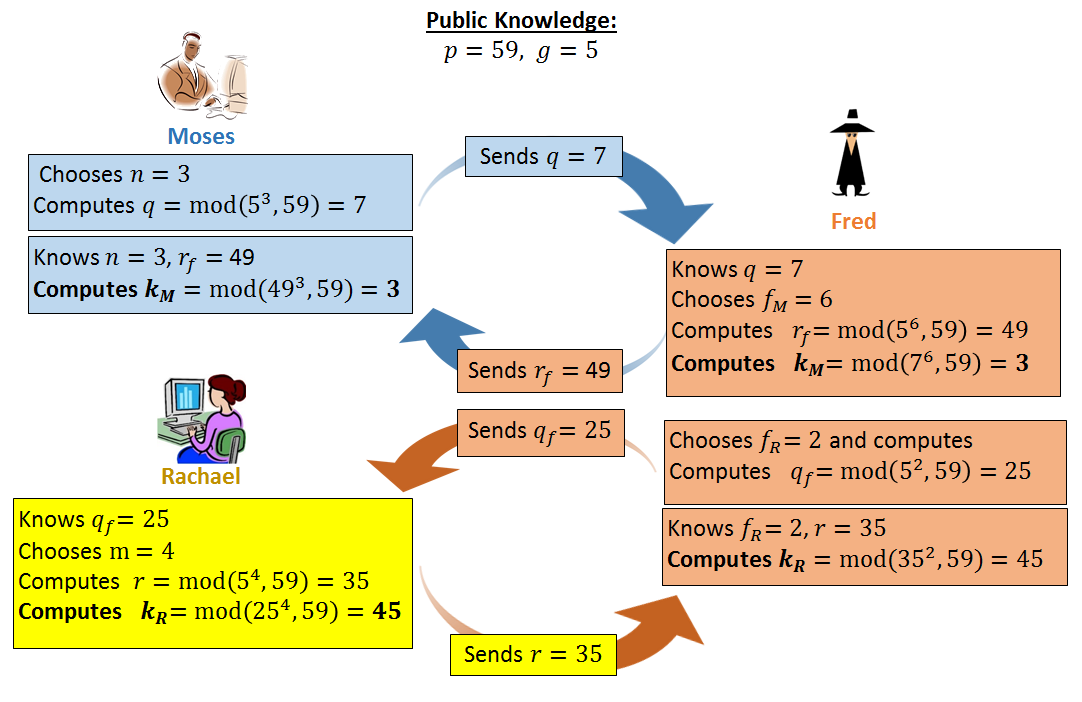
\includegraphics[width=5in]
	         {images/DHKE_18.png}}
	  \caption{\label{fig:DH:DHKE_2} MiM Attack during Moses and Rachael's Key Exchange }
\end{figure}

Following Figure~\ref{fig:DH:DHKE_2}, Fred establishes a secret key $k_M$ with Moses and another secret key $k_R$ with Rachael.  Now Moses thinks he has Rachael's public key, and Rachael thinks that she has Moses' public key. Moses and Rachael both combine their private keys with Fred's public keys and create two different symmetric keys, $K_M$ and $K_R$ respectively. At this point if Moses or Rachael sends a message then Fred is free to decrypt and encrypt the message using the appropriate symmetric key. 

DHKE is vulnerable to this type of MiM attack since Moses cannot verify that Rachael was the originator of the message, and vice-versa.  Preventing a MiM is difficult, but you can overcome a MiM attack using a \term{digital signature}, a digital signature is an electronic signature that encrypts data.  This digital signature serves two purposes: first, it authenticates the origin of the sender and second, it ensures the integrity of the message.  Generally in RSA, a public key is used to encrypt and a private key is used to decrypt (see Section \ref{sec:RSA}.  However, the reverse is more secure.  A message is encrypted using the private key and is decrypted using a public key (asymmetric cryptography). Although digital signatures cannot prevent eavesdropping, they can ensure that false messages are not authenticated. In the next section, we'ill examine the second of these alternatives. 

\section{Elliptic Curve Cryptography}\label{sec:ECC:2}

Elliptic Curve Cryptography (ECC) is one approach to the public key sharing dilemma that offers a smaller security level-to-key lenth ratio (see table below for the relationship  of security and key lengths).  In a cryptosystem the key length is the number of bits in the key (in DHKE the size of the symmetric key is $K1$).  For comparison a 160 bit key has 49 decimal digits, while a 1024 bit key has 309 decimal digits. 

The strength of a cryptography security level is also measured in bits (80, 128, 192, 256, etc.), and each security bit represents the number of computational steps necessary to find a solution.  For example, a security level of 80 means that $2^{80}$ computations are required to break the code. Referencing the table below, we can see that ECC with a 160 bit Finite Field has a similar security level to RSA and Diffie Hellman with 1024-bit moduli. To give you an idea of security level strength, "in 2002 it took $10^4$ computers (mainly PCs) running 24 hours a day for 549 days" to solve an EC with a 109 bit key length. 
\begin{figure} [H]
	   \center{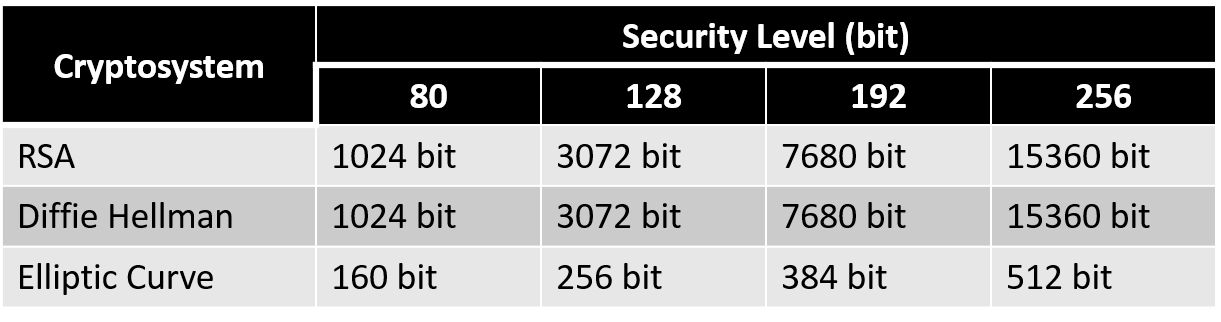
\includegraphics[width=5in]
	         {images/DHKE_9.png}}
	  \caption{\label{fig:DH:DHKE_9} Key bit lengths of Cryptosystems for different security levels recommended by the National Institute of Standards and Technology, retrieved from 
\url{http://resources.infosecinstitute.com/ecc-case-mobile-encryption/}}
\end{figure}
Now that we have established that elliptic curves provide more security with a smaller key size, lets examine the type of elliptic curves we need to use.

\subsection{Elliptic Curves}
An elliptic curve is an algebraic curve defined by the equation, $y^2 = x^3 + ax + b$.  See Figure~\ref{fig:DH:DHKE_5} below for different geometrical representations of elliptic  curves.  
\begin{figure}[H]
	   \center{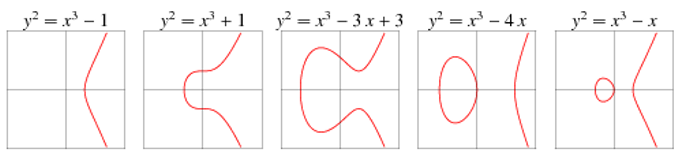
\includegraphics[width=5in]
	         {images/DHKE_5.png}}
	  \caption{\label{fig:DH:DHKE_5}  Geometric shapes of elliptic curves }
\end{figure}
Additionally, the Elliptic Curve (EC) is not allowed to have a double or triple root.  A triple root produces a singularity in the graph, and a double root produces a self-intersection (see graphs in Figure~\ref{fig:DH:DHKE_10}).  It turns out that we can guarantee that the EC has no double or triple roots if the coefficients $a$ and $b$ satisfy the following equation: $4a^3 + 27b^2 \neq 0$.  See graphs in Figure~\ref{fig:DH:DHKE_10} for a geometrical representation.
\begin{figure}[H]
	   \center{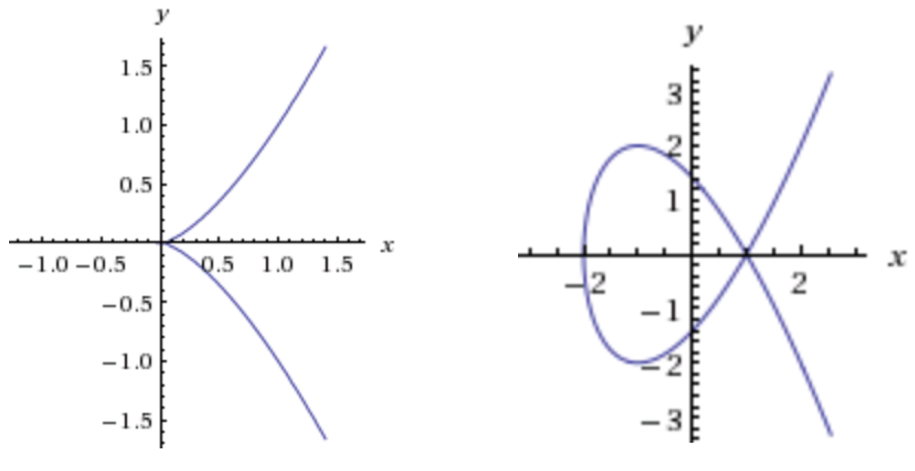
\includegraphics[width=3in]
	         {images/DHKE_10.png}}
	  \caption{\label{fig:DH:DHKE_10} E: $ y^2$ = $x^3$ and E: $ y^2$ = $x^3+ax+b$ }
\end{figure}
\begin{exercise}{}
		\begin{enumerate}[(a)] 
	\item  Prove that if the equation $y^2 = x^3 + ax + b$ has a double root or triple root, then $4a^3+27b^2=0$. (Hint:  if there's a double root , then it must be the case that $0 = x^3 + ax + b$ has a double root. This means that the equation can be factored:  $x^3 + ax+b = (x-r_1)^2(x-r_2)$.  See if you can express $r_1$ and $r_2$ in terms of $a$ and $b$.)\\
	\item Show that if $4a^3 + 27b ^2=0$, then the equation has a double root.  (Hint: there are 2 cases: (i) $b=0$, (ii) $b \neq 0$. In the case $b \neq 0$, first, show that $a > 0$.  Then use part (a) to express $r_1$ and $r_2$ in terms of $a$ and $b$, and show the equation factors properly.
\end {enumerate} 
\end{exercise}

Elliptic curves with coefficients in $\mathbb{R}$ are not used in practical applications, because it is impossible for computers to compute decimal fractions exactly.  The next section will discuss the elliptic curve group.

\subsection{Elliptic Curve Groups}
Given the right type of EC we can use the shape of the EC to conduct specific mathematical operations. A group operation, within the parameters of the EC, is sometimes referred to as addition and is given by two points on the EC, $P_1$, $P_2$ $\in$ E then $P_1 + P_2$ = $P_3$ .  The elements of the group are the points on the elliptic curve.  See below for the EC Group Properties.

\begin{enumerate}[1.]
\item \textbf{Identity}: There is no point on the curve that can serve as a neutral or identity element.  So we artificially define a point at infinity, to serve as the identity element, and it will be directly vertical of the point. 
\begin{figure}[H]
	   \center{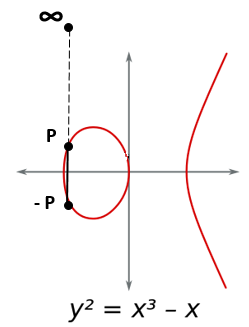
\includegraphics[width=2.5in]
	         {images/DHKE_13.png}}
	  \caption{\label{fig:DH:DHKE_13} Identity property for EC}
\end{figure}
\item \textbf{Inverse}: If you draw a line connecting $\infty$ with $P_1$ the intersection is $-P_1$. So, given a point $P$, the inverse is the point symmetric about the x-axis. 
\begin{figure}[H]
	   \center{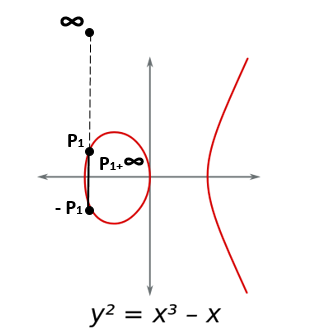
\includegraphics[width=2.5in]
	         {images/DHKE_14.png}}
	  \caption{\label{fig:DH:DHKE_14} Inverse property for EC }
\end{figure}
\item \textbf{closure}: if $P_1$ and $P_2$ are points on the elliptic curve the $P_1 + P_2$ is also a point on the curve;
\item \textbf{associativity}:$(P_1 + P_2) + P_3 = P_1 + (P_2 + P_3)$;
\begin{figure}[H]
	   \center{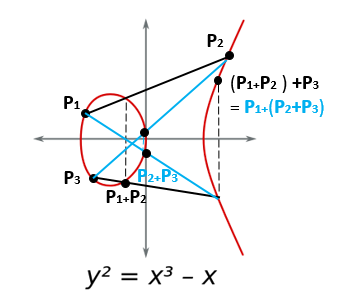
\includegraphics[width=4in]
	         {images/DHKE_12.png}}
	  \caption{\label{fig:DH:DHKE_12} Associative property for EC}
\end{figure}
\end{enumerate}

\begin{eg} Given E: $y^2 = x^3 + 2x + 2 (\bmod17)$, $P_1 = (5,1)$, $P_2 = (5,1)$, and $P_3 = (x_3, y_3)$
	Find $P_3$, where $P_3 = P_1 + P_2$
		\begin{align*}
		\textrm{(1) The slope~} m
		 &= ( (3 \cdot 5^2) + 2) \cdot (2 \cdot 1)^{-1} \bmod 17\\
	          &= (77) \cdot (2)^{-1} \bmod 17\\
                     &\equiv (9) \cdot (9) \bmod 17\\
                     &\equiv 81 \bmod 17\\
                    &\equiv 13
		\end{align*}
		\begin{align*}
		\textrm{(2)~}x_3
		 &= ( (13^2 - 5 - 5  (\bmod 17)) \text{\qquad \qquad \qquad \quad \: \: }\\
	          &= 159(\bmod 17)\\
                     &\equiv 6
		\end{align*}
			\begin{align*}
		\textrm{(3)~}y_3
		 &= ( (13(5 - 6) - 1(\bmod 17)) \text{\qquad \qquad \qquad \quad }\\
	          &= -14(\bmod 17)\\
                     &\equiv 3
		\end{align*}
Thus, $P_3 = (6,3) = 2P$
\end{eg}
\begin {exer}
Using Example 10, find the following: $3P, 4P, 5P, ..., 20P.$  Recall: $3P = 2P + P;  4P = 3P +P;$ etc.  What do you notice about $18P,  19P,$ and $20P?$
\end{exer}
Using Example 10 and Exercise 11, let us reconstruct the Diffie Hellman Key Exchange, but this time we'll use the strength of ECC.  Follow along with Figure~\ref{fig:DH:DHKE_8} below.

\begin{exer}
Using Example 10 and Exercise 11, what is the shared key exchange if Moses chooses $n = 9$ and Rachael chooses $m = 3$?
\end{exer}
\begin{figure}[H]
	   \center{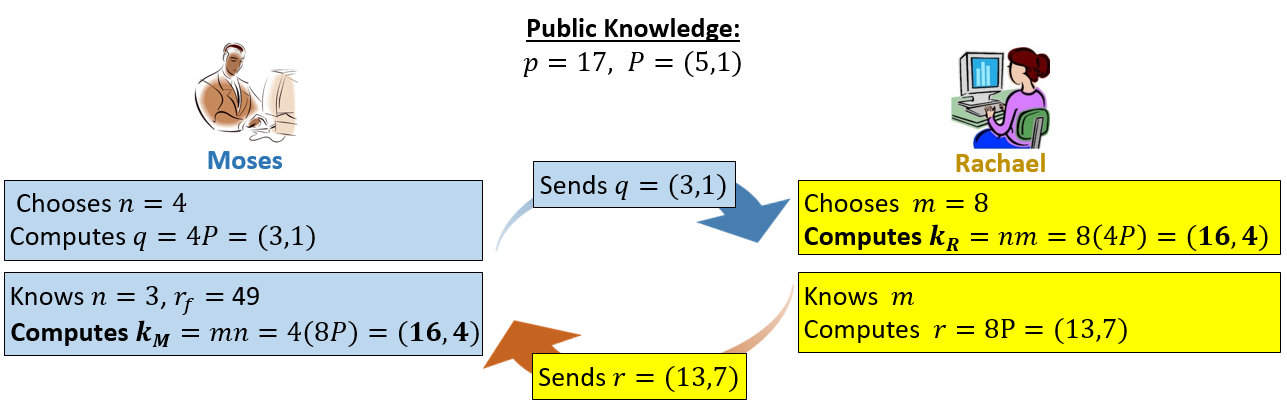
\includegraphics[width=5in]
	         {images/DHKE_8.png}}
	  \caption{\label{fig:DH:DHKE_8} Elliptic Curve Key Exchange between Moses and Rachael }
\end{figure}


\subsection{Elliptic Curve Math}
The elliptic curve protocol is how we perform calculations on the elliptic curve group. First, you must begin from a known point on the elliptic curve called the $generator$.  This point generates the next point which generates the point after that, and the point after that, and so on.  When performing EC math their are two scenarios.  The first is point 1 and point 2 are the same, $P1 = P2$, we'ill talk about how to do this computation a little later on. The second is $P1 \neq P2$. Geometrically if the two points are different then $P_1 + P_2$ is given by drawing a line from point $P_1$ to point $P_2$ and continue the line until it intersects the elliptic curve then reflecting that point about the $x$-axis.  See figure Figure~\ref{fig:DH:DHKE_6} below for a geometric representation.

\begin{figure}[H]
	   \center{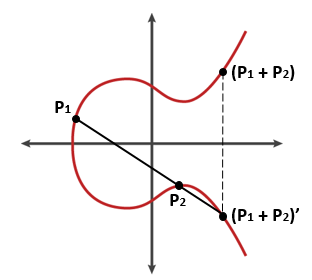
\includegraphics[width=2.5in]
	         {images/DHKE_6.png}}
	  \caption{\label{fig:DH:DHKE_6} Adding  two distinct points, $P_1 + P_2$ on the EC}
\end{figure}

When using Elliptic Curve Cryptography (ECC), the public key is the point on the elliptic curve, and the private key is the number of iterations or "hops" the generator must make to arrive at the public key point.  

It is important to note that $P_1 + P_2$ is always defined on the EC, even though sometimes it may not be apparent.  For instance, take E: $ y^2$ = $x^3 - x$, and points $P_1 = (2, \sqrt{6})$ and $P_2 = (3, \sqrt{24})$.  Then $P_1 + P_2 = (53.65,-377.18)$. See figure Figure~\ref{fig:DH:DHKE_16} below for a graphical representation.
\begin{figure}[H]
	   \center{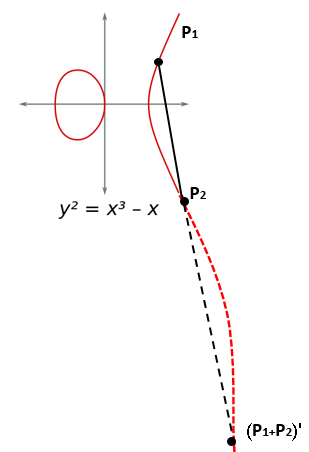
\includegraphics[width=2in]
	         {images/DHKE_16.png}}
	  \caption{\label{fig:DH:DHKE_16} $P_1 + P_2$ is always defined on the EC}
\end{figure}
Given E: $y^2 = x^3 + ax + b$, $P_1 = (x_1, y_1)$, $P_2 = (x_2, y_2)$, and $P_3 = (x_3, y_3)$. Find $P_3$, where $ P_3 =  P_1 + P_2$
\begin{enumerate}[(1)] 
	\item The slope $m =(y_2 - y_1)$ $\cdot$ $(x_2- x_1)^{-1}$, for $P_1$ $\neq$ $P_2$ \\
			\text{ \qquad \: \: \:}or $m = (3x_1^2 + a)$ $\cdot$ $(2y_1)^{-1}$, for $P_1 = P_2$ (this is found by finding\\
			\text{ \qquad \: \: \:}the first derivative of $f(x)$ and plugging the $x$ value into $f'(x)$ \\
			\text{ \qquad \: \: \:}to find the slope at the point)\\
	\item Plug values of $x_2$, $y_2$, and $m$ back into $m =(y_2 - y_1)$ $\cdot$ $(x_2- x_1)^{-1}$ in order to find equation of the line that passes through the two points \\
	\item Use the equation of the line and the equation of the EC to solve for ($x_3, y_3$)
\end {enumerate} 

\begin{eg} Given E: $y^2 = x^3 - 2x$, $P_1 = (0,0)$, $P_2 = (-1,1)$
	Find the line that passes through $P_1 + P_2$
		\begin{enumerate}[(1)] 
	\item The slope $m =(1 - 0)$ $\cdot$ $(-1- 0)^{-1}$ \\
		\text{ \qquad \: \: \:} =$(1)$ $\cdot$ $(-1)^{-1}$ \\
		\text{ \qquad \: \: \:} =-1 
	\item The line through $P_1 + P_2$ \\
		\text{ \qquad \: \:} recall: $y^2 = x^3 - 2x$ \\
		\text{ \qquad \: \:} $y - 1$ = $-1(x- 0)$ \\
		\text{ \qquad \: \:} $y$ =$-x + 1$ 
\end {enumerate} 
\end{eg}

\begin{eg} Given E: $y^2 = x^3 - x$, $P_1 = (2, \sqrt{6})$, $P_2 = (3, \sqrt{24})$ from figure Figure~\ref{fig:DH:DHKE_16} above.
	Find $P_3$, where $P_3 = P_1 + P_2$
		\begin{enumerate}[(1)] 
	\item The slope $m =(\sqrt{6} - \sqrt{24})$ $\cdot$ $(2- 3)^{-1}$ \\
		\text{ \qquad \: \:} or $m = -3\sqrt{6}$ 
	\item $y + \sqrt{24} = -3\sqrt{6}(x - 3)$ \\
		$y = -3\sqrt{6}x + 7\sqrt{6}$
	\item $0 = (-3\sqrt{6}x + 7\sqrt{6})^2 + x^3 - x$\\
		$x \approx 53.65, y \approx -377.18$\\
		$P_3 \approx (53.65, -377.18)$
\end {enumerate}  
\end{eg}

If the two points are the same, $P_1 = P_2$, then a tangent line to the point is drawn and the point of intersection to the EC is then reflected about the x-axis.  This is often referred to as point doubling. See Figure~\ref{fig:DH:DHKE_7} below for a geometrical representation.
\begin{figure}[H]
	   \center{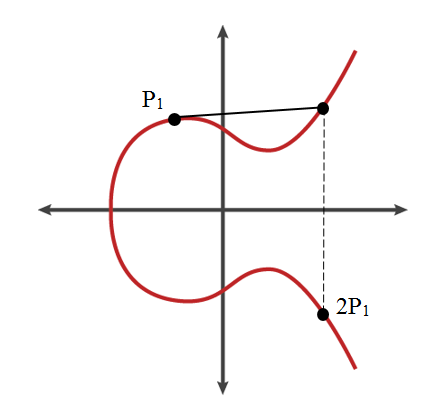
\includegraphics[width=2.5in]
	         {images/DHKE_7.png}}
	  \caption{\label{fig:DH:DHKE_7} Point doubling, adding one point to itself on the EC}
\end{figure}
\subsection{Galois Field} 
As a review, there are three types of algebraic structures: groups, rings, and fields (see Figure~\ref{fig:DH:DHKE_3}); each structure building from the previous structure.  Each structure is defined as a set of elements where: the given operation is closed, has the identity element, has the inverse element, and is associative. For the purpose of this text we'ill focus on Finite Fields (FF), which is a field that contains a finite number of elements and is also known as Galois Fields (GF). Applications of Galois Fields can be seen in CD players, DVD players, disk storage systems, and apps found on computers, tablets and smart phones.
\begin{figure}[H]
	   \center{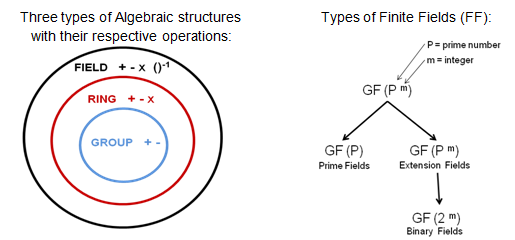
\includegraphics[width=4.5in]
	         {images/DHKE_3.png}}
	  \caption{\label{fig:DH:DHKE_3} Algebraic structures and types of FFs }
\end{figure}
 GFs only exist if they have $P^m$ elements, $GF(P^m)$. So, there is a GF with 27 elements $GF(27) = GF(3^3)$, there is a $GF$ with 256 elements $GF(256) = GF(2^8)$, etc.  In EC we are interested in Binary Fields (BFs), GFs of order $2^m$, with $m ≥ 1$.  Operations in the BF are defined in terms of an irreducible polynomial with degree $m$, this polynomial is also referred to as the reduction polynomial.  This means that the binary polynomial cannot be factored as a product of binary polynomials of degree less than $m$.  There are always $2^m$ elements in $GF(2^m)$, below is an example of the elements in $GF(2^3)$.  
\newline \newline
\begin{eg} Below are the 8 elements of $GF(2^3)$:
\begin{align*}
0, \quad 1, \quad X, \quad X +1, \quad X^2, \quad X^2+1, \quad X^2 + X, \quad X^2 + X + 1
 \end{align*}
\text{Adding two polynomials in $GF(2^3)$ is as follows:}
\begin{align*}
	f(x) &= X^2 + X\\
	g(x) &= X^2  + 1\\
           f(x) + g(x) &= X  + 1
 \end{align*}
 \text{Notice that the addition of the coefficient $X^2$ and the constant 1 = 0 in GF($2^3$)}
\end{eg}
\begin{rem} Given the polynomials $a,b \in  GF(P) = (0,1,2,...,P-1)$ then 
\begin{align*} 		
		a + b &\equiv c (\bmod P)\\
		a - b &\equiv d (\bmod P)\\
		a \cdot b &\equiv e (\bmod P) \quad \text{ ,the multiplicative group does not include 0}\\
		a^{-1} &\equiv b, \mathrm{~if~} \bmod (ab, P) = 1
\end{align*}
\end{rem}	
\begin{exer} Given $GF(2^4)$, add the following two polynomials:
\begin{align*}
	f(x) &= X^3 + X^2 + X + 1\\
	g(x) &= X^2  + 1
 \end{align*}
\end{exer}

\begin{exer} Given $GF(2^8)$, subtract the following two polynomials, $f(x) - g(x)$:
\begin{align*}	
	f(x) &= X^8 +         X^6 +          X^3 + X^2 + 1\\
	g(x) &=        X^7 + X^6 + X^5 +          X^2
\end{align*}
\end{exer}
\begin{rem}
Notice that the binary field has only two coefficients (0,1) so subtraction and addition are the same.
\end{rem}
\begin{eg}Given $GF(2^4)$ and the reduction polynomial $X + 1$, then adding two polynomials is as follows:
\begin{align*}	
	f(x) &=  X^2 + 1\\
	g(x) &= X^3 + X^2 + X + 1\\
	f(x) + g(x) &= X^3 + X (\bmod X + 1)\\
	&= 2X \text{( see below for explanation)}
\end{align*}
\begin{center}
\begin{tabular}{rrcrcrcr}
        &  $x^2$  &  $-$       &$x$&            \\ \cline{2-8}
 \multicolumn{1}{r|}{$x + 1$}
        &  $x^3$  &  $+$  &    &  $+$  & $ x$  \\
        & $x^3$   &  $+$  &    $x^2$ \\ \cline{2-8}
        &         &       &    $-$     $x^2$  &   $+$ &  $x$\\
        &         &       &    $-$     $x^2$  &  $-$  &   $x$  \\ \cline{4-8}
        &         &       &                    &          &   $2x$    &&
\end{tabular}
\end{center}
\end{eg}
\begin{eg} Given $GF(2^4)$ and the reduction polynomial $X^4 + X + 1$, then multiplying two polynomials is as follows:
\begin{align*}	
	f(x) &=  X^2 + X + 1\\
	g(x) &= X^3 + 1\\
 f(x) \cdot g(x) &= X^5 + X^4 + X^3 + X^2 + X + 1 (\bmod X^4 + X + 1)\\ 
	       &= - X^3 - X \text{ , is the remainder (see below for explanation) }
\end{align*}
\begin{center}
\begin{tabular}{rrcrcrcrcrcr}
        &  $x$  &  $+$  &      $1$         \\ \cline{2-12}
 \multicolumn{1}{r|}{$x^4 + x + 1$}
        &  $x^5$  &  $+$  &  $x^4$  &  $+$  & $ x^3$  &  $+$  &  $x^2$  &  $+$  & $ x$  &  $+$  &  $1$  \\
        & $x^5$   &  $+$  &       	&          &      	  &          &  $x^2$   & $+$  &  $x$     \\ \cline{2-12}
        &         &       &         $x^4$  & $+$   &  $ x^3$  &   $+$  &             &         &         &          &  $1$  \\
        &         &       &         $x^4$  &  $+$  &             &           &              &         &  $x$   & $+$  &  $1$   \\ \cline{4-12}
        &         &       &                    &          &   $x^3$ &    $-$  &              &         &  $x$    
\end{tabular}
\end{center}
\end{eg}
We proved the following in Exercise~\ref{exercise:modular:71}.

\begin{prop}{BezoutsIdentity}(\emph{Bezout's Identity})~~ let $x$ and $t$ be two-non-zero integers, and let $d$ be their GCD, then there exists integers $p$ and $a$ such that\\
 \hspace*{\parindent} $px + at = d$
\end{prop}

\begin{corollary}
Using Bezout's Identity we can conclude that if $p$ and $a$ are coprime then we have\\
\hspace*{\parindent} $px + at = 1$ \\
reducing $\bmod p$ yields $at = 1 \bmod p$ .  So $t$ is the multiplicative inverse of\\
 $a$ $\bmod n$.
\end{corollary}

\begin{eg} Given $GF(2^8)$ and the reduction polynomial $X^8 + X^4 + X^3 + X +1$, and $a$ = $X^6 + X^4 + X + 1$ then finding the multiplicative inverse of $a$ is as follows:  $a^{-1}$ = $b$, if $a$ $\cdot$ $b$ $(\bmod p)$ = $1$ .  To find $a^{-1}$ use the Extended Euclidian Algorithm.
\\
	$p =  X^8 + X^4 + X^3 + X +1$\\ 
	$a = X^6 + X^4 + X + 1$\\
\\Using the quotients and remainders found below, we can find the multiplicative inverse of $a$ using the following steps \\(new $t$ = old $t - $quotient $\cdot$ $t$):
\begin{enumerate}
\item $t = 0$
\item new $ t = 1$ 
\item new $t = 0 - 1\cdot(x^2 + 1)$
\item  new $t = 1 - (x^4 + x^2)\cdot(x^2 + 1)$
\item new $t = (x^2 + 1) - (x+1)\cdot(x^6 + x^2 + 1)$
\item Stop here and simplify, since the subsequent remainder is 0.
\item new $t = (x^2 + 1) - (x+1)\cdot(x^6 + x^2 + 1)$ = $x^7 + x^6 + x^3 + x$
\end{enumerate}
Thus, $a^{-1}$ = $x^7 + x^6 + x^3 + x$\\
\begin{center}
\begin{tabular}{rrcrcrcrcrcrcr}
        &  $x^2$  &  $+$  &      $1$         \\ \cline{2-14}
 \multicolumn{1}{r|}{$x^6 + x^4 + x + 1$}
        &  $x^8$  &  $+$  &    &      &  $x^4$  &  $+$  & $ x^3$  &  $+$  &   &   & $ x$  &  $+$  &  $1$  \\
        & $x^8$   &  $+$  &    $x^6$      &    $+$         &      &     &  $x^3$  &  $+$  & $x^2$        \\ \cline{2-14}
        &         &              &$x^6$ &$+$ &  $x^4$  & $+$   &              &          & $ x^2$  &   $+$  & $x$   &  $+$  & $1$       \\
        &         &              &$x^6$ &$+$ &  $x^4$  & $+$   &              &          &   &    & $x$   &  $+$  & $1$   \\ \cline{4-14}
        &         &               &          &      &             &           &       &     & $x^2$ 
\end{tabular}
\end{center}

\begin{center}.

\begin{tabular}{rrcrcrcrcrcrcr}
        &  $x^4$  &  $+$  &      $x^2$      \\ \cline{2-8}
 \multicolumn{1}{r|}{$x^2$}
        &  $x^6$  &  $+$  &    $x^4$  &  $+$   & $ x$  &  $+$  &  $ 1$  \\
        & $x^6$     \\ \cline{2-8}
        &              &           &     $x^4$   & $+$  & $x$   &  $+$   & $1$   \\ 
        &              &           &     $x^4$    \\ \cline{4-8}  
        &              &           &                  &          &  $ x$  &  $+$  &  $ 1$  \\
\end{tabular}
\end{center}

\begin{center}
\begin{tabular}{rrcrcrcrcrcr}
        &  $x$  &  $+$  &      $1$      \\ \cline{2-6}
 \multicolumn{1}{r|}{$x + 1$}
        &  $x^2$  \\
        & $x^2$   &  $+$  &    $x$  \\ \cline{2-6}
        &             &          &    $x$   \\
        &             &          &    $x$  & $+$ & $1$ \\ \cline{4-6}
        &             &          &           &        &  $1$
\end{tabular}
\end{center}

\begin{center}
\begin{tabular}{rrcrcrcrcrcr}
        &  $x$  &  $+$  &      $1$      \\ \cline{2-4}
 \multicolumn{1}{r|}{$1$}
        &  $x$      &   $+$ &    $1$  \\
        & $x$     \\ \cline{2-4}
        &             &          &    $1$   \\
        &             &          &    $1$ \\ \cline{3-4}
        &             &          &    $0$
\end{tabular}
\end{center}

\end{eg}

\begin{exer}
What are the binary elements of GF($2^4$)?
\end{exer}
\begin{exer}
Given GF($2^{12}$), then adding $f(X)$+ $g(X)$ = ?
        \\ $f(X)$ = $X^{10} + X^8 + X^5 + X + 1$
        \\ $g(X)$ = $X^{10} + 1$
\end{exer}
\begin{exer}
Given GF($2^4$), then adding $f(X)$ + $g(X)$ = ?
        \\ $f(X)$ = $X^{2} + X $
        \\ $g(X)$ = $X^{3} + 1$
\end{exer}
\begin{exer}
Given GF($2^5$), then subtracting $f(X)$ + $g(X)$ = ?
        \\ $f(X)$ = $X^{4} + X^2 + 1 $
        \\ $g(X)$ = $X^{3} + 1$
\end{exer}
\begin{exer}
Given GF($2^7$), then subtracting $f(X)$ + $g(X)$ = ?
        \\ $f(X)$ = $X^{6} + X^4 + X $
        \\ $g(X)$ = $X^{3} + 1$
\end{exer}
\begin{exer}
Given GF($2^5$) and the reduction polynomial $X^5 + X + 1$ , then multiplying two polynomials, $f(X)$ $\cdot$ $g(X)$ = ?
        \\ $f(X)$ = $X^{3} + X + 1 $
        \\ $g(X)$ = $X^{4} + X$
\end{exer}
\begin{exer}
Given GF($2^5$) and the reduction polynomial $X^5 + X + 1$ , then multiplying two polynomials, $f(X)$ $\cdot$ $g(X)$ = ?
        \\ $f(X)$ = $X^{4} + X^3 + 1 $
        \\ $g(X)$ = $X^{4} + X^2 + X + 1$
\end{exer}
\begin{exer}
Given GF($2^{160}$) and the reduction polynomial $X^{160} + X + 1$ , then multiplying two polynomials, $f(X)$ $\cdot$ $g(X)$ = ?
        \\ $f(X)$ = $X^{120} + X^{100} + 1 $
        \\ $g(X)$ = $X^{80} + X^{70} + X^{60}$
\end{exer}

\subsection{Elliptic Curve Integrated Encryption System} 
If Moses and Rachael would like to communicate a message using ECC, then they could use an agreed-upon code table and elliptic curve.  Each character of the encrypted message would correspond to a point on the elliptic curve $E_p(a,b)$ where $p$ is a prime number, and Rachael and Moses will have to choose a random point $C$ and $B$ respectively on the EC. Additionally, Rachael selects a random number $\alpha$ which is less than the order of $E_p(a,b)$ and a point $A$ on the EC. She computes $A_1 = $$\alpha$ $(C + A)$ and $A_2= $$\alpha$$A$. Rachael's private keys are $\alpha$ and the point $A$; her public keys are $A_1$ and $A_2$. Moses does the same thing but using $\beta$ and a point $B$. Rachael's public key for Moses is $A_B = $$\alpha$$B_2$, and Moses' public key for Rachael is $B_A = $$\beta$$A_2$. Now lets consider an elliptic curve whose equation is $y^2 = x^3 + 2x + 9$ to see how this works, see Figure~\ref{fig:DH:DHKE_11} below.

\begin{figure}[H]
	   \center{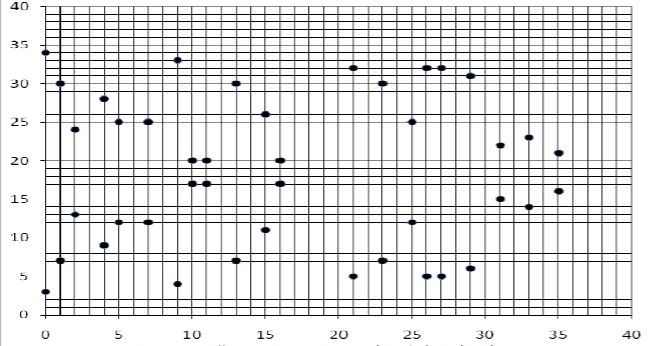
\includegraphics[width=1.5in]
	         {images/DHKE_11.png}}
	  \caption{\label{fig:DH:DHKE_11} Elliptic Curve, $y^2 = x^3 + 2x + 9$ }
\end{figure}

If we choose $37$ as our prime number $p$ then we'll restrict ourselves to the Finite Field, $FF(37)$, so ($y^2 = x^3 + 2x + 9$)$\bmod37$ and use $E_{37}(2,9)$.  Then the points on the elliptic curve are as followed:
($\infty, (5, 25), (1, 30), (21, 32), (7, 25), (25, 12), (4, 28), (0, 34), (16, 17), (15, 26), (27, 32), \newline(9, 4), (2, 24), (26, 5), (33, 14),(11, 17), (31, 22), (13, 30), (35, 21), (23, 7), (10, 17), (29, 6), \newline(29, 31), (10, 20), (23, 30), (35, 16), (13, 7), (31, 15), (11, 20), (33, 23), (26, 32), (2, 13), (9, 33), \newline(27, 5), (15, 11), (16, 20), (0, 3), (4, 9), (25, 25), (7, 12), (21, 5), (1, 7), (5, 12)$)

We can now assign each point on the EC to a character of our choosing and create a code table that will be known to the sender and receiver. Using the table seen in Figure~\ref{fig:DH:DHKE_17} below, Moses and Rachael can now communicate any message to each other.  

\begin{figure}[H]
	   \center{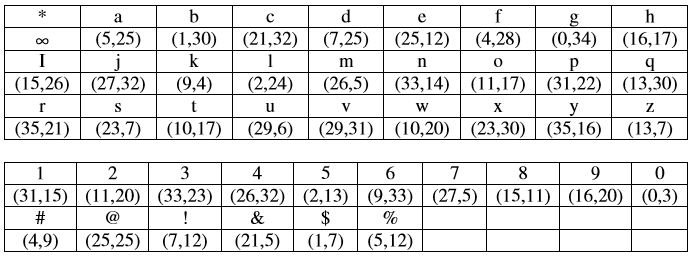
\includegraphics[width=6in]
	         {images/DHKE_17.png}}
	  \caption{\label{fig:DH:DHKE_17} Code table using the EC agreed upon by Moses and Rachael }
\end{figure}

In order for Moses to Encrypt a mesage "M" all of the characters must correspond to points on the EC using the agreed upon table.  The result is a pair of cipher points $(E_1, E_2)$.  Moses chooses a random number, $\gamma$ which changes for each point. So,
$E_1 =$$\gamma$$C$, and $E_2 = M +($$\beta$ $+$$\gamma$$)$$A_1 -$$\gamma$$A_2 + A_B$. After encrypting all characters Moses then converts the pair of points into the text characters using the code table and communicates this message to Rachael.\\

After receiving the cipher text Rachael will decrypt the message using:\\
$M = E_2 - ($$\alpha$ $E_1 +$$\alpha$$B_1 +B_A)$\\

\begin{eg} Moses will send the message, ``attack" using the code table above.\\
First, Rachael and Moses must establish their private and public keys.\\
Rachael lets $C = (9,4)$ and $\alpha$ $= 5$ and $A = (10, 20)$ on the EC. These are her private keys.\\
	$A_1 = 5[(9, 4) + (10, 20)] = (1, 7)$, public key\\
	$A_2 = (32, 23)$, public key\\ \\
Moses lets $B = (11, 20)$ and $\beta$ $= 7$. These are his private keys. \\
	$B_1 = (11, 17)$, public key\\
	$B_2 = (23, 30)$, public key

\begin{flushleft}
Now Moses must encrypt his message one character at a time.
\end{flushleft}
\begin{enumerate}[(1)] 
\item Moses chooses $\gamma$$ = 8$ and encrypts the letter ``a" \newline
	So, the point $(5, 25)$ is encrypted as\newline
	$E_1 = $$\gamma$$C = (1, 30)$ which corresponds to the letter ``b" since $C$ is in the 11th position in the generated table and $\bmod(8 \cdot 11,43) = 2$ and the second position is the character ``b". \newline
	$E_2 = M +($$\beta$ $+$$\gamma$$)$$A_1 -$$\gamma$$A_2 + A_B$ \newline
	$= (5, 25) + 15(1, 7) - 8(32, 23) + (15, 11)$ \newline
	$= 1 + 13 - 17 + 34 = 31\mod 43 = 31 = (2, 13)$ which corresponds to ``5" in the code table.  So, ``a" is encrypted as $(b, 5)$
\item Moses chooses $\gamma$$ = 12$ and encrypts the letter ``t" \newline
	So, the point $(10, 17)$ is encrypted as\newline
	$E_1 = $$\gamma$$C = (21, 32)$ which corresponds to the letter ``c"\newline
	$E_2 = M +($$\beta$ $+$$\gamma$$)$$A_1 -$$\gamma$$A_2 + A_B = (2, 24)$ which corresponds to ``l" in the code table.  So, ``t" is encrypted as $(c, l)$
\item Moses chooses $\gamma$$ = 19$ and encrypts the letter ``t" \newline
	So, the point $(10, 17)$ is encrypted as\newline
	$E_1 = $$\gamma$$C = (4, 9)$ which corresponds to the ``$\#$"\newline
	$E_2 = M +($$\beta$ $+$$\gamma$$)$$A_1 -$$\gamma$$A_2 + A_B = (27, 32)$ which corresponds to ``j" in the code table.  So, ``t" is encrypted as $($$\#$$, j)$
\item Moses chooses $\gamma$$ = 2$ and encrypts the letter ``a" \newline
	So, the point $(5, 25)$ is encrypted as\newline
	$E_1 = $$\gamma$$C = (29, 31)$ which corresponds to the letter ``v"\newline
	$E_2 = M +($$\beta$ $+$$\gamma$$)$$A_1 -$$\gamma$$A_2 + A_B = (1, 30)$ which corresponds to ``b" in the code table.  So, ``a" is encrypted as $(v, b)$
\item Moses chooses $\gamma$$ = 3$ and encrypts the letter ``c" \newline
	So, the point $(5, 25)$ is encrypted as\newline
	$E_1 = $$\gamma$$C = (1, 30)$ which corresponds to the letter ``b"\newline
	$E_2 = M +($$\beta$ $+$$\gamma$$)$$A_1 -$$\gamma$$A_2 + A_B = (31, 22)$ which corresponds to ``p" in the code table.  So, ``c" is encrypted as $(b, p)$
\item Moses chooses $\gamma$$ = 23$ and encrypts the letter ``k" \newline
	So, the point $(9, 4)$ is encrypted as\newline
	$E_1 = $$\gamma$$C = (25, 25)$ which corresponds to ``@"\newline
	$E_2 = M +($$\beta$ $+$$\gamma$$)$$A_1 -$$\gamma$$A_2 + A_B = (4, 28)$ which corresponds to ``f" in the code table.  So, ``a" is encrypted as $(@, f)$
\end{enumerate}
\begin{flushleft}
"attack" is communicated to Rachael as the cypher $(b,5; c,l; $$\#$$,j; v,b; b,p; @,f)$. Rachael is now able to decrypt the cypher text by first converting the characters to their corresponding points, and then uses them to decrypt $M$.
\end{flushleft}
\begin{enumerate}[(1)]
\item $M = E_2 - ($$\alpha$ $E_1 +$$\alpha$$B_1 +B_A) = (5, 25)$ which corresponds to the character ``a" in the code table.\newline
\item $M = E_2 - ($$\alpha$ $E_1 +$$\alpha$$B_1 +B_A) = (10, 17)$ which corresponds to the character ``t" in the code table.\newline
\item $M = E_2 - ($$\alpha$ $E_1 +$$\alpha$$B_1 +B_A) = (10, 17)$ which corresponds to the character ``t" in the code table.\newline
\item $M = E_2 - ($$\alpha$ $E_1 +$$\alpha$$B_1 +B_A) = (5, 25)$ which corresponds to the character ``a" in the code table.\newline
\item $M = E_2 - ($$\alpha$ $E_1 +$$\alpha$$B_1 +B_A) = (21, 32)$ which corresponds to the character ``c" in the code table.\newline
\item $M = E_2 - ($$\alpha$ $E_1 +$$\alpha$$B_1 +B_A) = (9, 4)$ which corresponds to the character ``k" in the code table.\newline
\end{enumerate}
\end{eg} 
It is important to choose a large prime number $p$, in order to make it difficult for an eavesdropper to crack your code.  Computers use a base-2 number system known as the binary number system.  Internet protocols usually use a minimum of a 1024-bit prime number for $p$, which is equivalent to $2^{1024}$ or 300 decimal digits long.  So, there are $2^{1023}$ different possibilities for 1024 bits (where the highest bit is a `1`). It is not necessary to generate your own prime.  There are many records of large primes published that can be referenced. For example, if you visit \url{https://primes.utm.edu/} you can see some lists of 210 digit primes and larger.

\newpage  

\subsection{References and Suggested Reading} 
\begin{enumerate}[(1)]

\item
Azad, Saiful, and Pathan, Al-Sakib Khan. "Elliptic Curve Cryptography" in Practical Cryptography, CRC Press, January 2015.

\item 
Bidgoli, Hossein. "Diffie-Hellman Key Exchange" in \emph{Handbook of Information \newline
Security: Information Warfare, Social, Legal, and International Issues and \newline
Security Foundations, Volume 2}, John Wiley and Sons, January 2006.

\item 
Bos, Joppe, Kaihara, Marcelo, Kleinjung, Thorsten, Lenstra,Arjen,and Montgomery, Peter. (2009, September 01). \emph{On the Security of 1024-bit RSA and 160-bit Elliptic Curve Cryptography}. Retrieved from \url{https://eprint.iacr.org/2009/389.pdf}.

\item 
Christensen, Chris. (2015, November 14). \emph{Key Exchanges}. Retrieved from \url{http://www.nku.edu/~christensen/092mat483}

\item
Franco, Pedro. "Elliptic Curve Cryptography" in \emph{Understanding Bitcoin: Cryptography, Engineering and Economics}, John Wiley and Sons, February 2015.

\item 
Kumar, Suneetha, Chandrasekhar. (2012, January). \emph{Encryption of Data  Using \newline
Elliptic Curve Over Finite Fields}. Retrieved from \newline 
\url{https://arxiv.org/ftp/arxiv/papers/1202/1202.1895.pdf}.

\item 
Mandal, Surajit, Manna, Nilotpal, and Saha, Arijit. "Diffie-Hellman \newline
Key Exchange" in \emph{Information Theory, Coding, and Cryptography}, Pearson India, May 2013.

\item 
Pomerance, Carls. (n.d.). \emph{Discrete Logarithms}. Retrieved from \url{https://math.dartmouth.edu/~carlp/dltalk09.pdf}.




\end{enumerate}